\chapter{\textcolor{myred}{Distribución binomial}}

\section{\huge{Introducción}}

\textcolor{myred}{\hrule}

\newthought{Consideremos}, una población de individuos que no se reproducen y evolucionan en tiempo discreto que evolucionan en tiempo discreto. A cada paso de tiempo cada uno de ellos puede morir con probabilidad $d$. Calcule numéricamente la distribución de probabilidad de la población en función del tiempo (para algunos tiempos, y para un par de valores de d). Compare con la distribución
binomial exacta

Realizamos simulaciones 














\begin{marginfigure}
\captionsetup{type=figure}
    \centering
    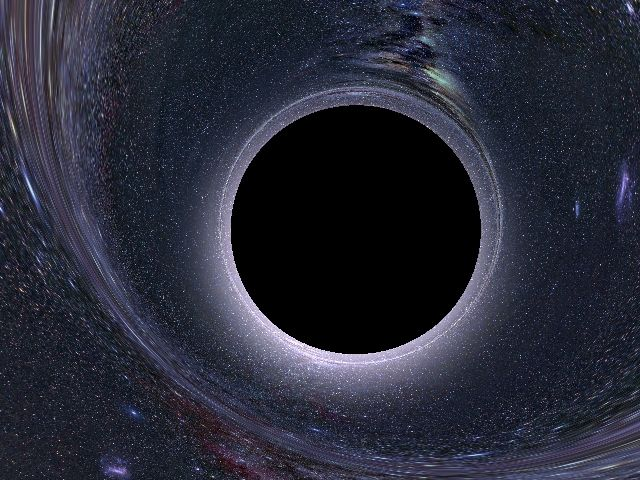
\includegraphics[width=1.3\textwidth]{Im/3653b705a42ad6a980fc834e6ca39875.jpg}
    \caption{Agujero negro de Reissner-Nordström, imagen generada por raytracing.}
    \label{fig:sen}
\end{marginfigure}

Es decir que, para cuando hallamos terminado el trabajo, tanto nosotrxs como lx lectorx deberá tener, al menos, una respuesta básica para las siguientes preguntas: ¿En qué consiste la Teoría General de la Relatividad?, ¿qué es la gravedad?, ¿qué es una métrica o un tensor métrico?, ¿qué significa que el espacio-tiempo esté 'curvado', y cómo puedo calcular dicha curvatura?, ¿cómo interviene la carga eléctrica en dicha curvatura?, ¿cómo son las trayectorias de partículas (neutras y cargadas) y de la luz, en un espacio-tiempo donde hay objetos con masa y carga eléctrica?
\begin{marginfigure}
\captionsetup{type=figure}
    \centering
    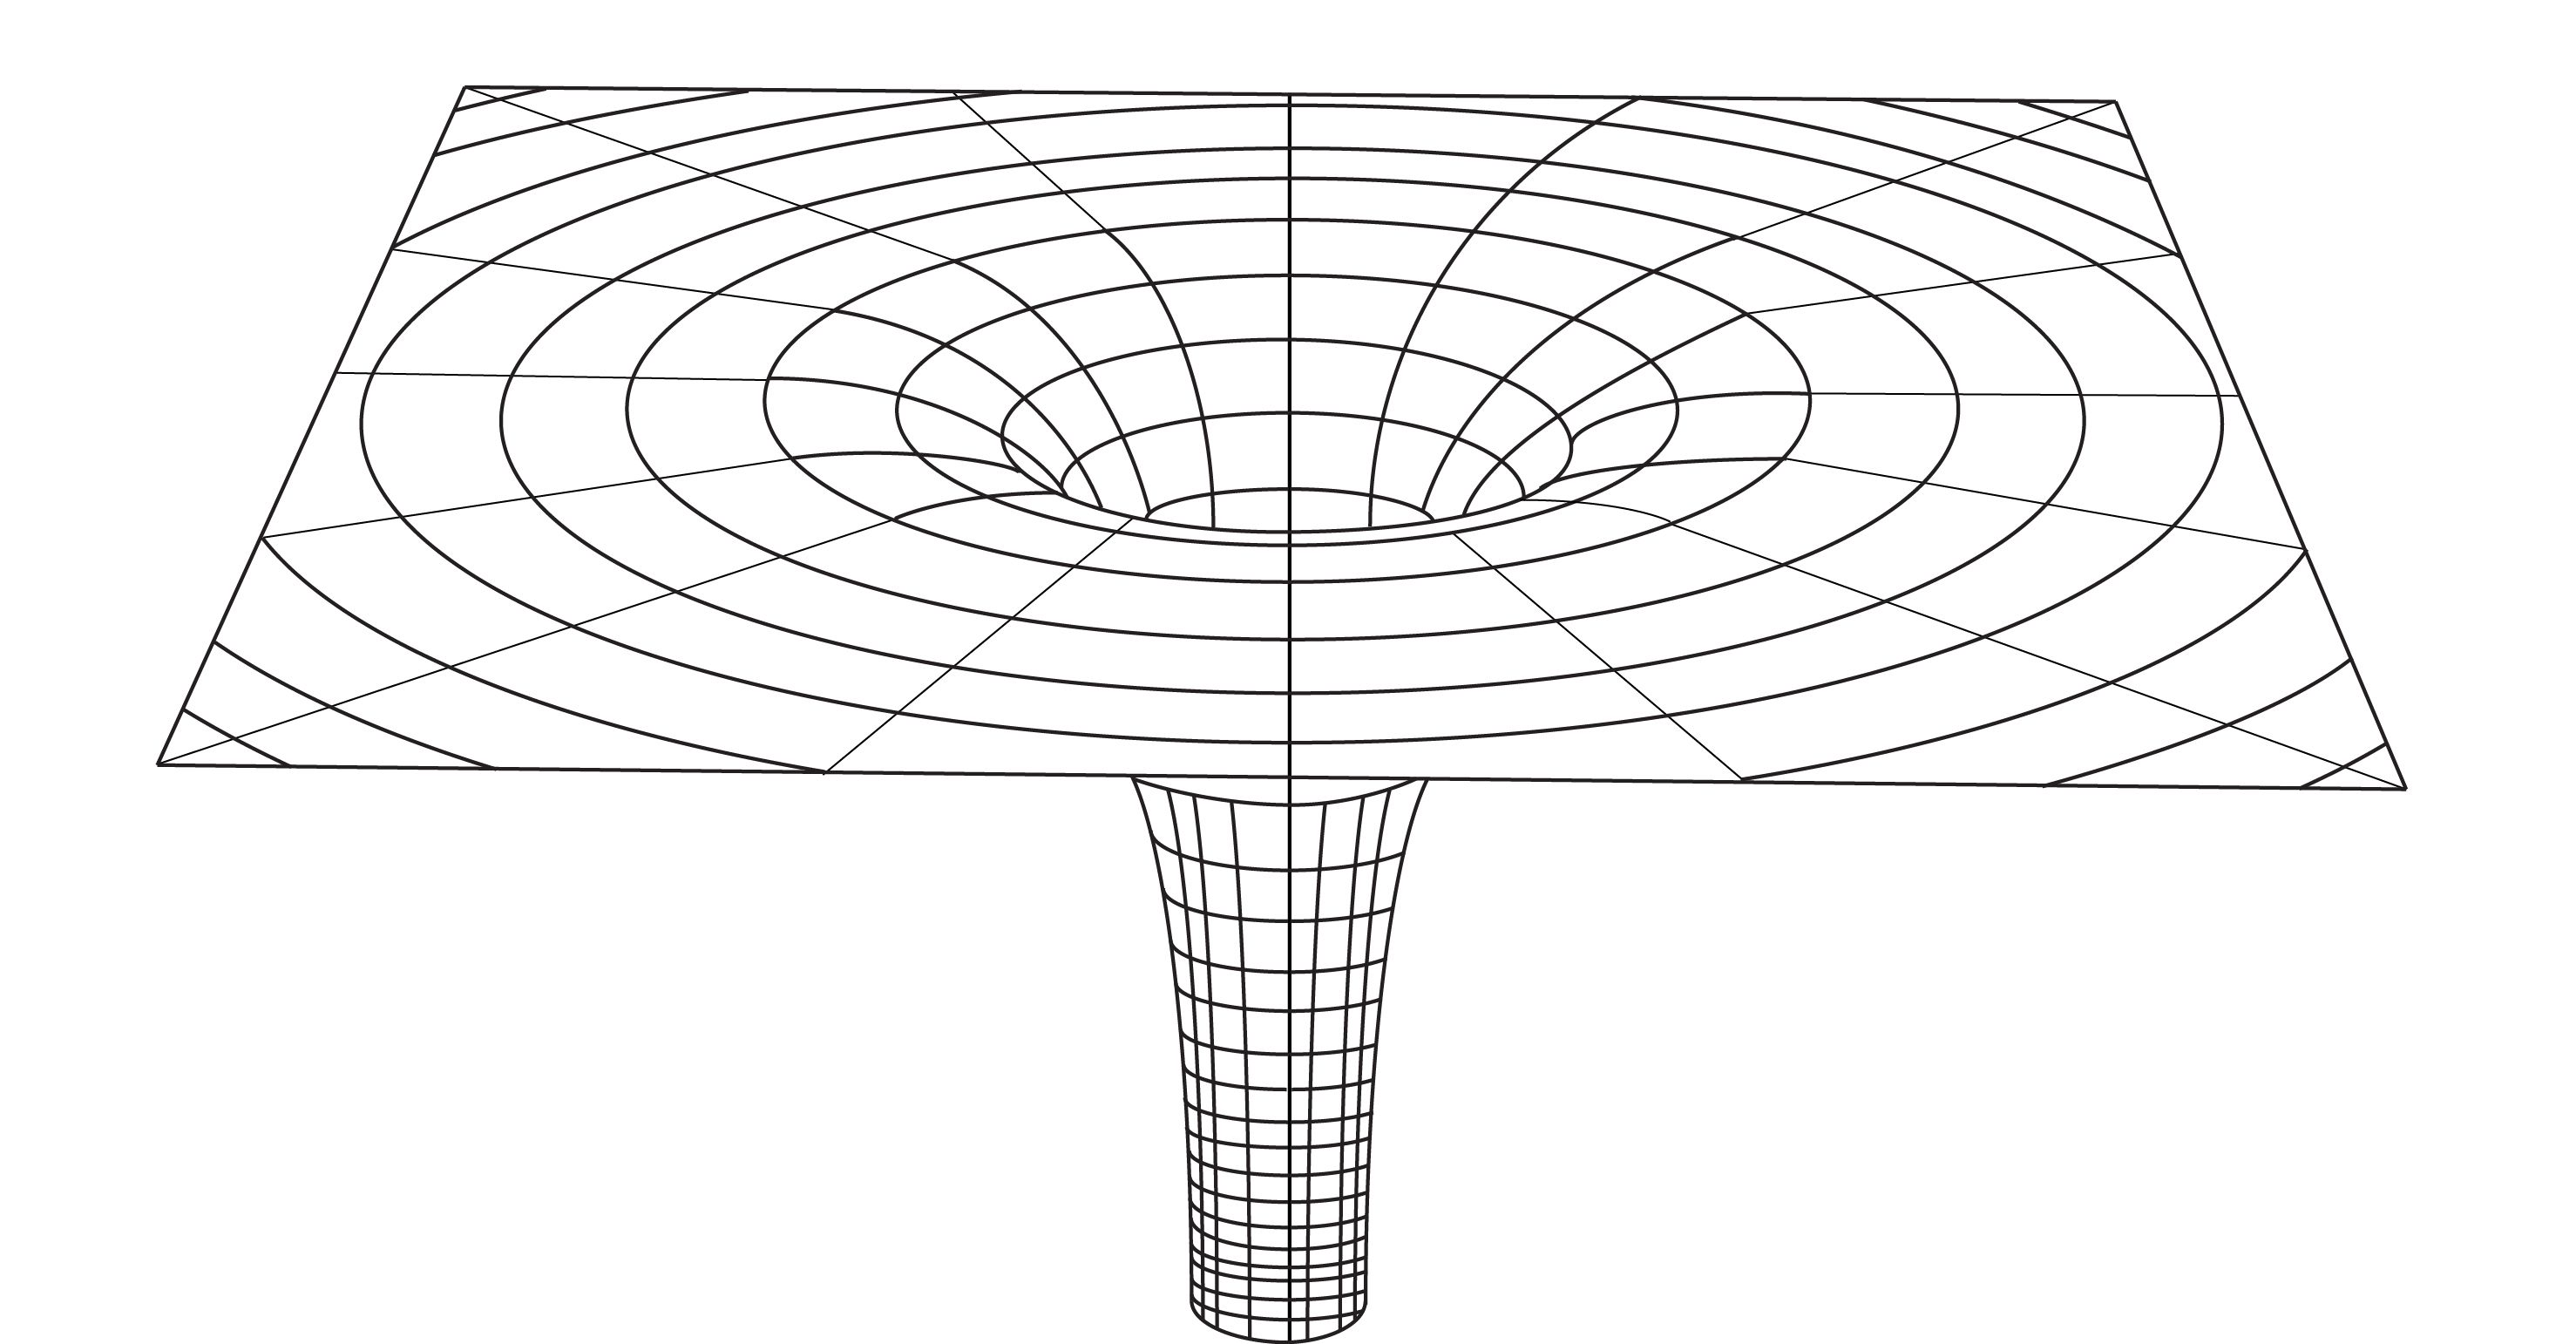
\includegraphics[width=1.3\textwidth]{Im/27c518672e8aa2b372107cca7726603f.jpg}
    \caption{Representación de un agujero negro.}
    \label{fig:sen}
\end{marginfigure}
Como siempre, es conveniente separar el trabajo en partes, y eso es lo que haremos aquí. Este documento consta entonces de cuatro capítulos y un epílogo:

\begin{remarkbox}{}
\begin{itemize}
    \item \textbf{Capítulo 1} - Teoría General de la Relatividad
    \item \textbf{Capítulo 2} - Ecuación de Campo de Einstein
    \item \textbf{Capítulo 3} - Métrica de Reissner-Nordström
    \item \textbf{Capítulo 4} - Simulaciones Computacionales
    \item \textbf{Epílogo} - Conclusiones, Fronteras y Bilbiografía
\end{itemize}
\end{remarkbox}

\section{\huge{GR in a nutshell}}
\textcolor{myred}{\hrule width\textwidth}

\begin{flushright}
\textit{Gravity is matter's response to loneliness.}\\ \textbf{Alice Wu}
\end{flushright}
\newthought{Sin más preámbulo}, comencemos \textit{spoileando} la Teoría General de la Relatividad (GR, por sus siglas en inglés). Para motivarnos, veamos primero la \textbf{Ley de Gravitación Universal} (Newton, 1687):

\begin{marginfigure}
\captionsetup{type=figure}
    \centering
    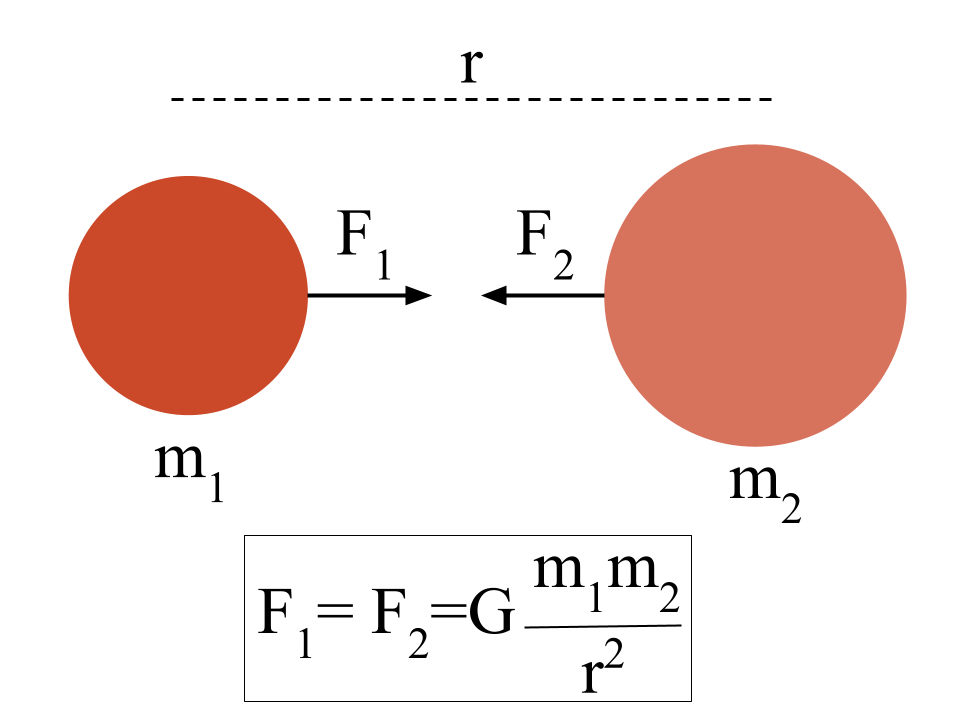
\includegraphics[width=1.3\textwidth]{Im/gravuniv.png}
    \caption{Ley de Gravitación Universal.}
    \label{fig:sen}
\end{marginfigure}

\begin{equation}
    F_{g}=G\frac{m_1 m_2}{r^2}
\end{equation}

Quien halla estudiado algo sobre la Teoría Especial de la Relatividad (SR), o esté familiarizadx con el fenómeno de \textbf{Retardación} del Electromagnetismo \footnote{\textbf{Retardation}, Cassinese F. y Lembo I. (2020)}, notará enseguida que esta ecuación no puede ser la explicación completa de la interacción gravitatoria: \textbf{el tiempo no aparece en ninguna parte}. Es decir que, por ejemplo, un cambio en la masa $m_1$ influiría \textbf{instantáneamente} en la masa $m_2$, y ya sabemos que en el mundo real casi nada es instantáneo. Claramente le falta algo a la teoría de Newton: explicar qué es la gravedad, cuál es el mecanismo según el cual los objetos con masa interactúan entre sí.

\newthought{Ahora bien,} ¿cuál es este mecanismo? Para dar con él, vamos a establecer dos relaciones fundamentales: primero, la \textbf{relación entre gravedad y aceleración}, y luego la \textbf{relación entre aceleración y curvatura}.


\begin{figure}[h!]
    \centering
    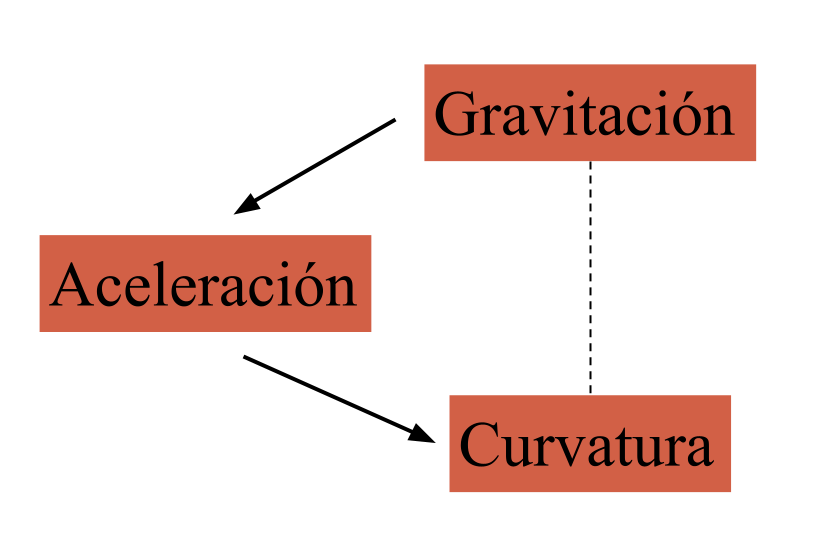
\includegraphics[width=0.7\textwidth]{Im/curvatura aceleracion.png}
    \label{fig:sen}
\end{figure}

\subsection*{\textbf{Gravedad y Aceleración}}

\begin{marginfigure}
\captionsetup{type=figure}
    \centering
    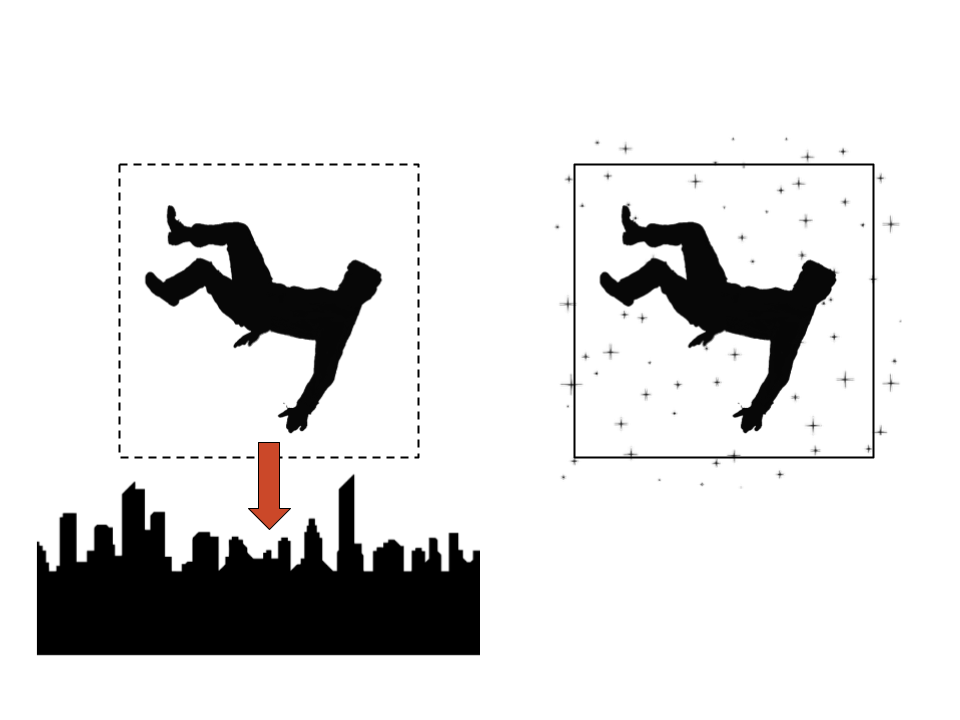
\includegraphics[width=1.3\textwidth]{Im/happiestthought.png}
    \caption{El pintor en caída libre no experimenta peso alguno, mientras cae siente lo mismo que si estuviera flotando libremente en el espacio.}
    \label{fig:sen}
\end{marginfigure}
En 1907, mientras trabajaba en una fábrica de patentes en Suiza, Einstein concibió lo que luego llamó su \textit{pensamiento más feliz}: al mirar por la ventana a un pintor en el exterior de un edificio, se imaginó qué sucedería si éste se cayera del andamio. Durante su caída, pensó, el pintor no experimentaría su propio peso (weightlessness). Es decir, en el sistema no-inercial solidario al pintor durante la caída desaparece la fuerza peso, podemos eliminar la interacción gravitatoria al considerar un sistema acelerado. Podemos decir que entonces \textbf{existe una analogía entre sistemas acelerados y sistemas bajo la influencia de campos gravitatorios}.

Esto es el llamado \textbf{Principio de Equivalencia}, sobre el cual hablaremos en detalle en la sección siguiente.

\subsection*{\textbf{Aceleración y Curvatura}}

Esta segunda relación es probablemente más difícil de comprender que la primera, principalmente porque aún no dimos una definición formal de curvatura en un espacio-tiempo. De momento, vamos a conformarnos con un ejemplo en el cual una medición realizada en un sistema inercial da un resultado distinto a una medición realizada en un sistema acelerado, anticipando que esta discrepancia en las mediciones guarda una estrecha relación con la definición de curvatura.

\begin{remarkbox}{Paradoja de Ehrenfest}
Consideremos un cilindro que rota uniformemente a velocidad $\omega$. Si realizamos una medición desde el sistema inercial del laboratorio, mediremos un radio $r$, y una circunferencia $c=2\pi r$.


Si, por otro lado, medimos desde un sistema solidario al cilindro, la \textbf{contracción de Lorentz} hará que las reglas del borde, que se mueven con velocidad tangencial a la circunferencia, se contraigan Tenemos que $c'>c=2\pi r$. Por otro lado, al medir el radio la velocidad es perpendicular a las reglas, y entonces $r'=r$.

Entonces, en nuestro sistema acelerado ya no vale que $c'=2\pi r'$. Esto ya nos puede dar una idea de que en un espacio curvado dejan de ser válidas las relaciones propias de la geometría euclidiana.

\end{remarkbox}
\begin{figure}
    \centering
    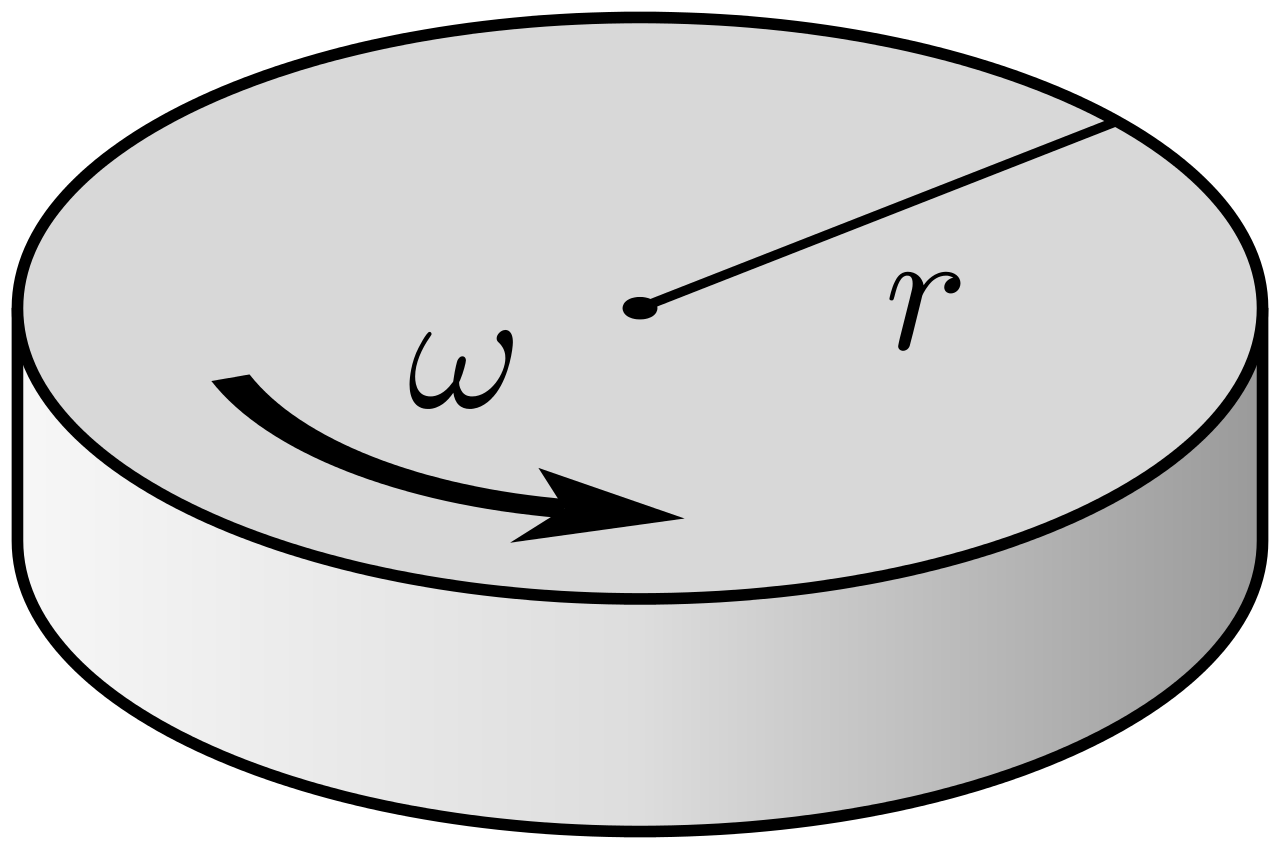
\includegraphics[width=0.315\textwidth]{Im/Spinning-disk.svg.png}
    \caption{Cilindro que rota con velocidad uniforme $\omega$.}
    \label{fig:sen}
\end{figure}

\begin{figure}
    \centering
    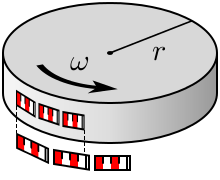
\includegraphics[width=0.3\textwidth]{Im/220px-Ehrenfest-paradox-disk.svg.png}
    \caption{Las reglas en el sistema laboratorio miden una circunferencia distinta a las del sistema no-inercial.}
    \label{fig:sen}
\end{figure}



¿Podemos concluir entonces que, mediante las dos relaciones establecidas, ya hemos vinculado interacción gravitatoria con curvatura del espacio-tiempo? Sí y no. Lo desarrollado es conceptualmente correcto, pero si queremos establecer una Teoría de la Relatividad General, donde Relatividad significa lo mismo que en Relatividad Especial, vamos a tener que \textbf{independizarnos de todo sistema de referencia}, incluidos los sistemas acelerados. Convencerse de esto ya es en sí mismo una tarea difícil (de hecho, le llevó a Einstein 7 años desprenderse de la idea de que las coordenadas nos dicen algo sobre el sistema estudiado\cite[][p.2-4]{wheeler}), pero además trae consigo la complicación de necesitar una formulación matemática que haga explícita esta independencia del sistema de coordenadas. Esto quiere decir que necesitamos una \textbf{formulación covariante} para las leyes, la cual se realiza a través de \textbf{tensores}\cite[][p.247]{landau2}.

Además, veremos que la equivalencia entre sistemas acelerados y gravitacionales es limitada: existen las denominadas \textbf{fuerzas de marea} (tidal forces), que nos imponen restricciones a la hora de construir nuestros sistemas. 

\begin{marginfigure}
\captionsetup{type=figure}
    \centering
    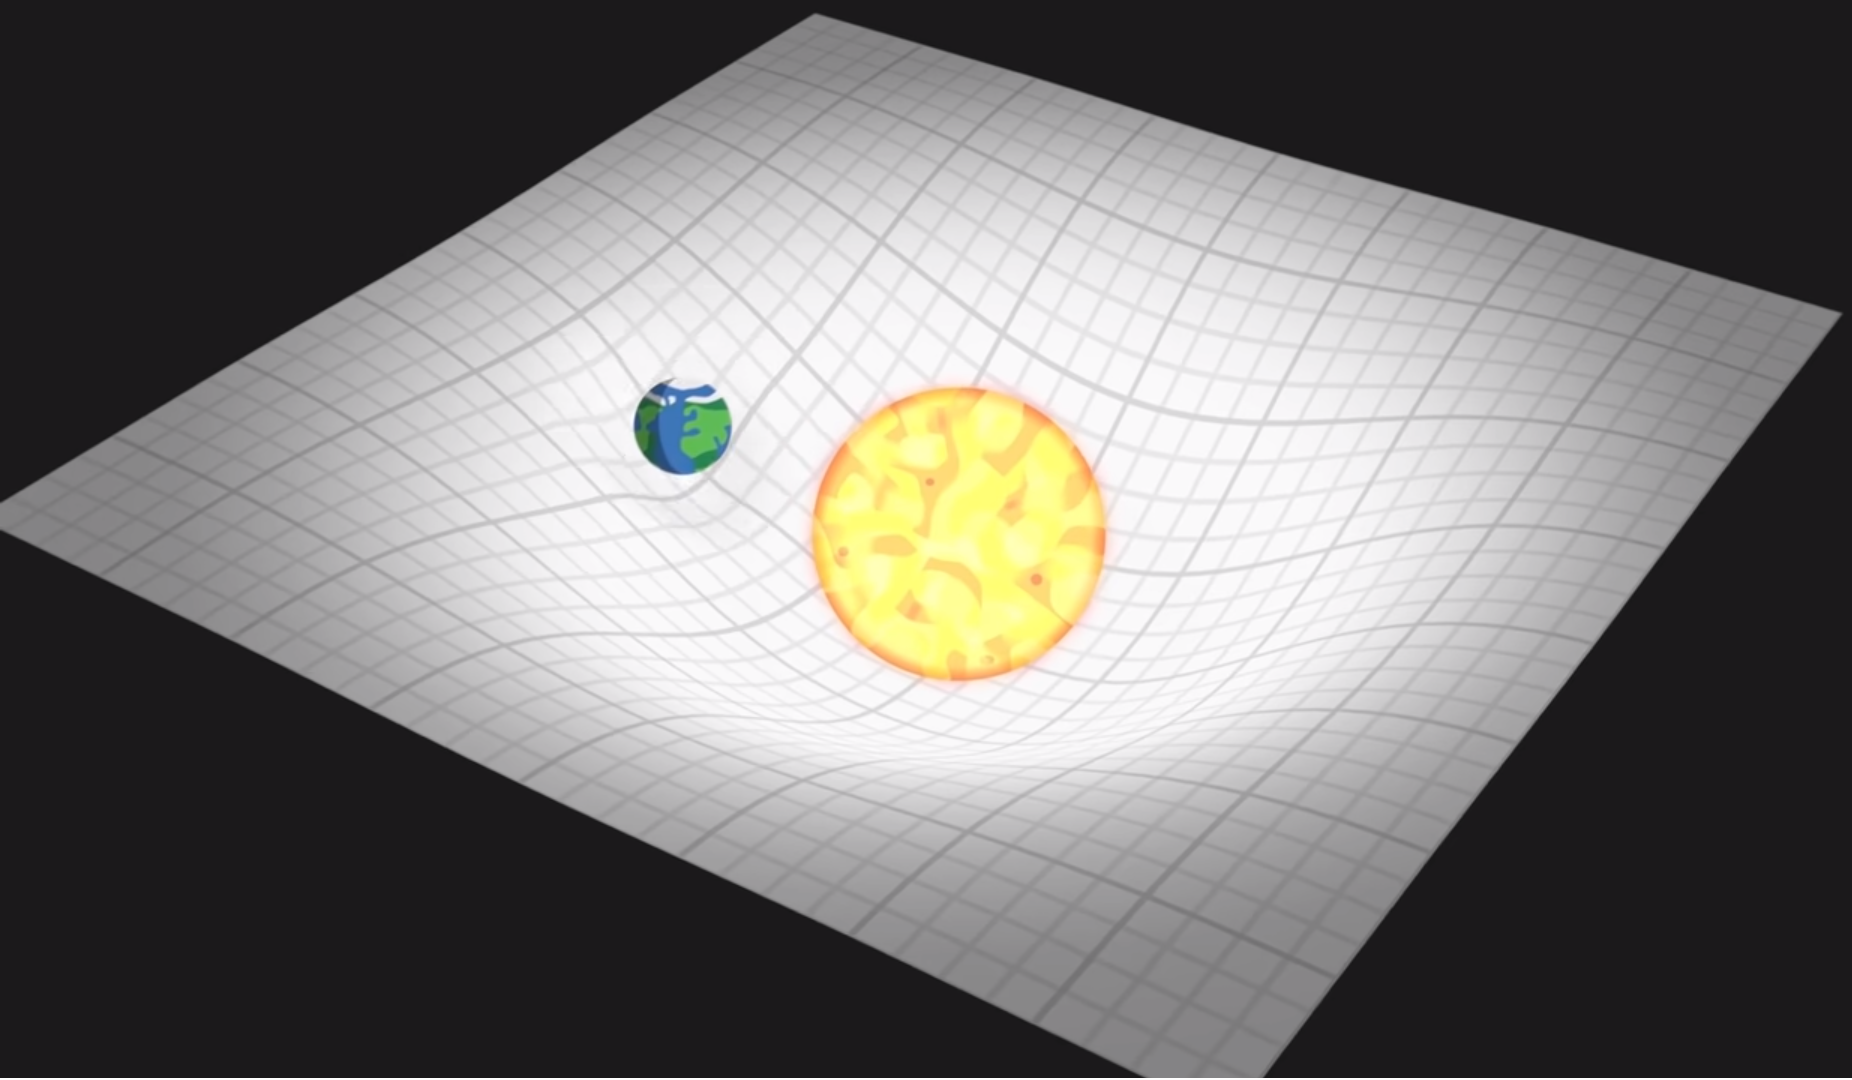
\includegraphics[width=1.3\textwidth]{Im/sistsolar.png}
    \caption{La masa del Sol curva el espacio-tiempo, y la Tierra se mueve en una geodésica a través de este espacio-tiempo curvado.}
    \label{fig:sen}
\end{marginfigure}

\newthought{Para concluir} con este breve resumen, mencionaremos la \textbf{hipótesis geodésica}, que en síntesis nos dice que \textbf{las partícula libres se mueven siguiendo una única trayectoria, denominada geodésica, que está definida por las características geométricas del espacio-tiempo.} Estas curvas pueden definirse como las líneas que \textbf{localmente más se asemejan a una recta}. Como estamos trabajando con un espacio-tiempo posiblemente curvo, las trayectorias muchas veces no se verán como líneas rectas, como es el caso de las órbitas de los planetas alrededor del Sol. 


\newpage

\section{\huge{Detalles del Principio de Equivalencia}}
\textcolor{myred}{\hrule width\textwidth}

\newthought{Volvamos a considerar} la Ley de Gravitación Universal, ahora con dos partículas de masas $M$ y $m_g$. Si incorporamos la Segunda Ley de Newton, tenemos que:

\begin{equation}
    F_g=G\frac{Mm_g}{r^2}=m_i a
\end{equation}

\begin{marginfigure}
\captionsetup{type=figure}
    \centering
    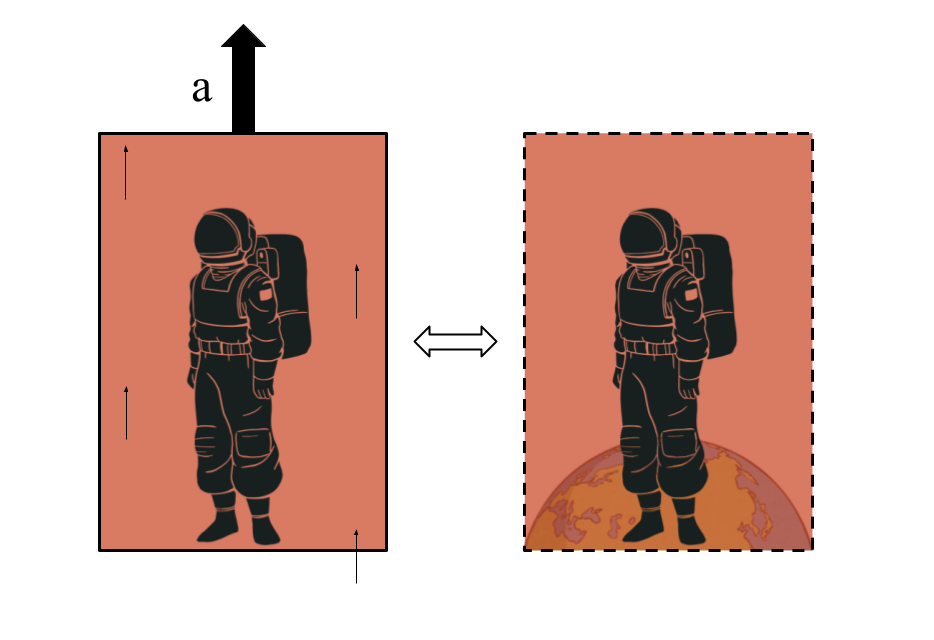
\includegraphics[width=1.3\textwidth]{Im/equiv.png}
    \caption{Principio de Equivalencia: lx cosmonauta o puede distinguir si está en un ascensor acelerándose hacia arriba en el espacio, o en un campo gravitatorio en reposo sobre la Tierra.}
    \label{fig:sen}
\end{marginfigure}

Donde $m_i$ es la \textbf{masa inercial} de la partícula, es decir, qué tanto 'se resiste' esta partícula a ser acelerada por una fuerza dada. Por otro lado, $m_g$ es la \textbf{masa gravitatoria}, la cual indica qué tan fuerte es la interacción de la partícula con un campo gravitatorio (de manera similar a la carga $Q$ en Electromagnetismo). Estos conceptos son \textbf{completamente diferentes}, y a priori no deberíamos esperar que estén relacionados entre sí\cite[][p.2]{moore}.

La experiencia demuestra que, en realidad, ambas masas sí son iguales, lo cual nos permite realizar la siguiente afirmación fundamental: \textbf{en un campo gravitacional, todos los cuerpos se mueven de la misma manera, independientemente de su masa.}

Es esta propiedad la que nos permite establecer la analogía entre campos gravitacionales y sistemas acelerados. Un ejemplo emblemático de esto es considerar un sistema alejado de cualquier campo gravitacional, que se acelera uniformemente a $9,8 m/s^2$. Unx observadorx en este sistema no tiene forma de reconocer si realmente se está acelerando, o si está 'en reposo' (es decir, en un sistema inercial) en la superficie de la Tierra.

\begin{figure}[h!]
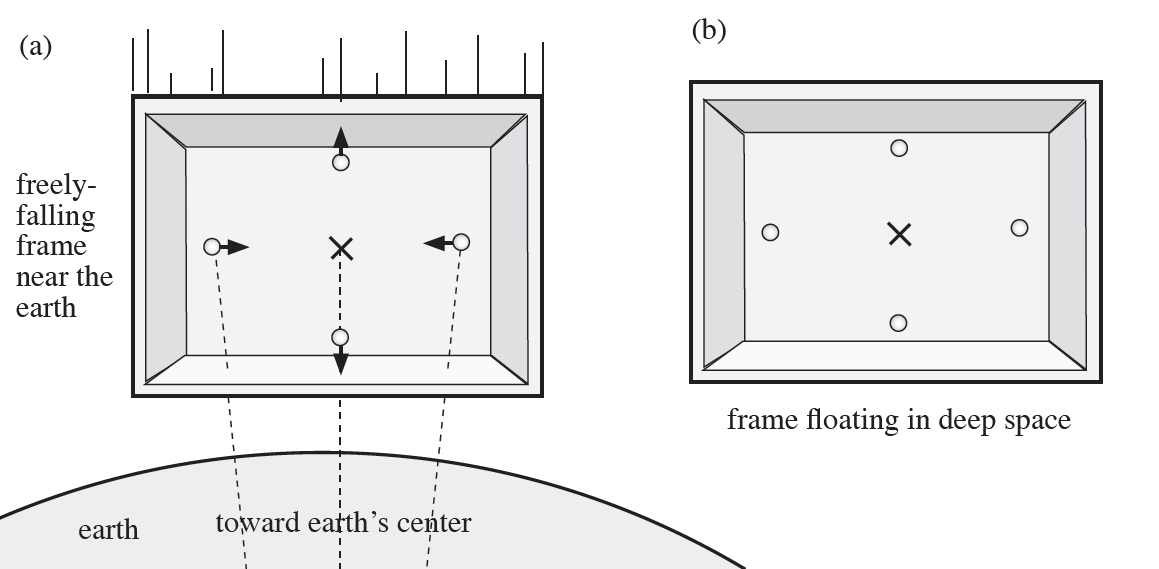
\includegraphics[width=\textwidth]{Im/tidal.png}
\caption{Si arrojáramos cuatro masas hacia la Tierra, la no-uniformidad del campo gravitatorio real haría que las masas de los costados se acerquen, y que las de arriba y abajo se alejen gradualmente. A esto se lo denomina \textbf{fuerzas de marea}, y no puede recrearse en un sistema que flota lejos de cualquier interacción gravitatoria.}
\label{fig:my_label}
\end{figure}

En realidad, lo enunciado anteriormente no es del todo cierto, por dos motivos:
\begin{itemize}
    \item Mientras que los campos gravitatorios \textit{siempre} tienden a cero al alejarse de la masa que los produce, los 'campos' asociados a sistemas acelerados no lo hacen. En el ejemplo recién mencionado, el 'campo' que mediría lx observadorx aceleradx sería igual en todos lados. En el ejemplo de la paradoja de Ehrenfest, la fuerza centrífuga que aparece en el sistema que rota se hace cada vez más grande a medida que nos alejamos del eje de rotación. 
    \item Los campos gravitatorios reales no son uniformes, por lo cual existen \textbf{fuerzas de marea} que tienden a comprimir o estirar cualquier cuerpo que se encuentre en ellos.
\end{itemize}

Es por esto que lo máximo que podemos hacer es, tomando un sistema no-inercial apropiado, eliminar el campo gravitatorio en una región lo suficientemente pequeña como para considerar al campo uniforme. El hecho de que los campos gravitatorios no puedan ser eliminados en su totalidad mediante la elección de un sistema de referencia, es una evidencia de la \textbf{realidad física} de los mismos.
\newpage
\section{\huge{Curvatura}}

\textcolor{myred}{\hrule width\textwidth}

\begin{flushright}
\textit{He visto a Lucy\\ Cuando entró a la habitación\\ El espacio se curvó}\\ \textbf{Gustavo Cerati}
\end{flushright}

\subsection*{\textbf{Coordenadas Curvilíneas}}
En esta sección, vamos a responder la ansiada pregunta: \textbf{¿qué es la curvatura?} Para ello, comencemos definiendo una \textbf{base de coordenadas} (Moore) o \textbf{coordenadas curvilíneas} (Landau). Sin importar qué tan complicado es nuestro espacio a considerar\footnote{Por simplicidad, de momento nos vamos a limitar a dos dimensiones $(u,w)$.}, siempre podemos definir\cite[][p.54]{moore}, en cada punto $\mathcal{P}$, un par de vectores $\mathbf{e}_u$ y $\mathbf{e}_w$ tales que:
\vspace{1cm}
\begin{fullwidth}
\begin{remarkbox}{Coordenadas Curvilíneas (en $2D$)}
\begin{itemize}
    \item $\mathbf{e}_u$ es tangente a la curva $w=cte$ y apunta en el sentido de $u$ creciente.
    \item $\mathbf{e}_w$ es tangente a la curva $u=cte$ y apunta en el sentido de $w$ creciente.
    \item Las longitudes de $\mathbf{e}_u$ y $\mathbf{e}_w$ son tales que el vector desplazamiento $d \mathbf{s}$ que va de $\mathcal{P}(u,w)$ a un punto infinitesimalmente cercano $(u+du,w+dw)$ puede escribirse como:
    $$d\mathbf{s}=du\mathbf{e}_u+dw\mathbf{e}_w=dx^{\mu}\mathbf{e}_{\mu}$$
\end{itemize}
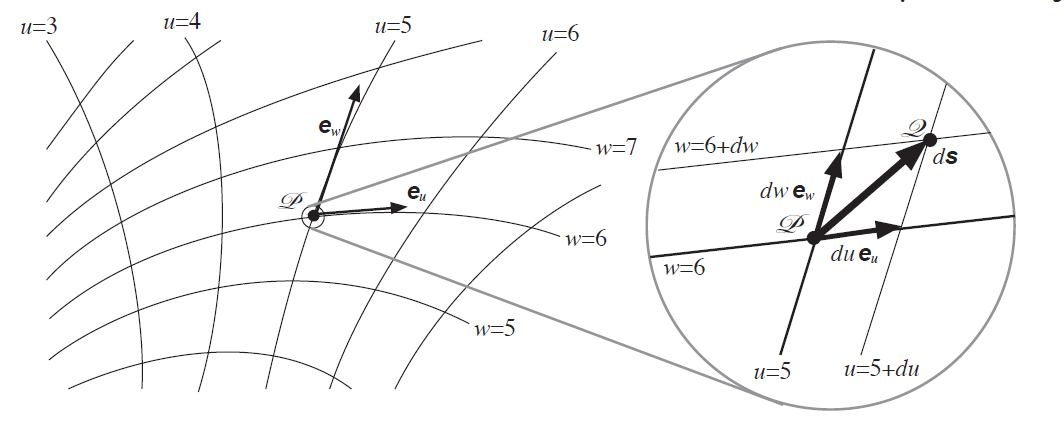
\includegraphics[width=1\textwidth]{Im/coord.png}
    \label{fig:sen}
\end{remarkbox}
\end{fullwidth}
Un sistema de coordenadas definido de esta manera puede resultar muy distinto a los versores cartesianos habituales, por los siguientes tres motivos: 

\begin{itemize}
    \item El producto escalar $\mathbf{e}_u \cdot \mathbf{e}_w$ puede ser \textbf{distinto de cero}.
    \item El módulo de $\mathbf{e}_u$ y $\mathbf{e}_w$ puede no ser igual a $1$.
    \item $\mathbf{e}_u$ y $\mathbf{e}_w$ pueden modificar sus módulos y/o direcciones a medida que nos movemos en el espacio.
\end{itemize}

\subsection*{\textbf{Tensor Métrico}}
\begin{marginfigure}
\captionsetup{type=figure}
    \centering
    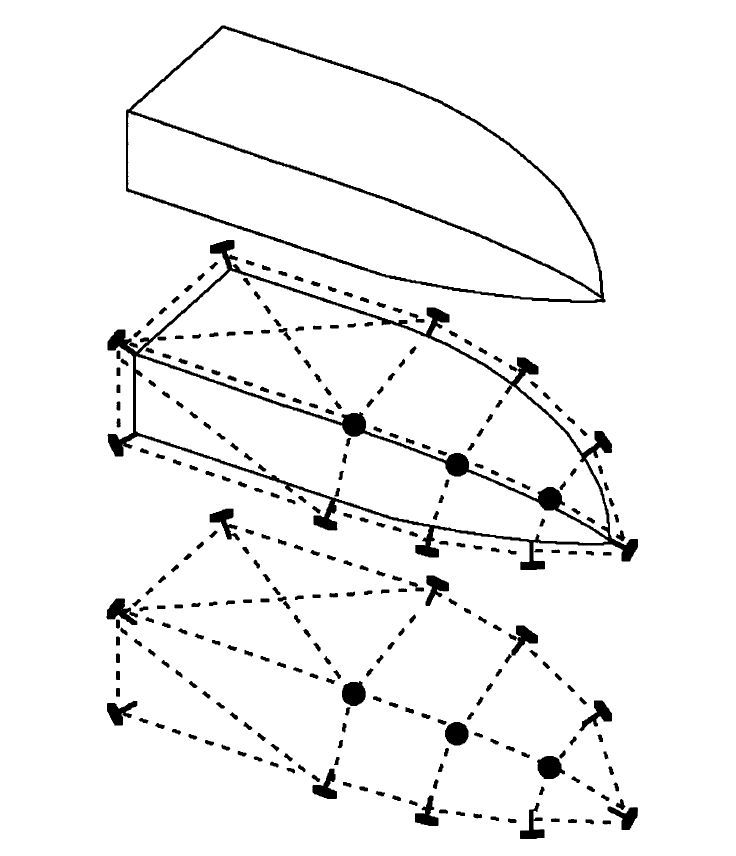
\includegraphics[width=1.3\textwidth]{Im/bote.png}
    \caption{Wheeler y Taylor explican que podemos estudiar la geometría de un espacio colocando 'clavos' (eventos) y anotando las distancias entre estos puntos.}
    \label{fig:sen}
\end{marginfigure}

Al igual que en Relatividad Especial, estamos interesadxs en estudiar \textbf{distancias entre eventos}, es decir, la separación espacial y temporal medida con reglas y relojes respecto a la cual todxs lxs observadorxs están de acuerdo: el \textbf{intervalo invariante}. En SR, ese intervalo se calculaba mediante:

\begin{equation}
    ds^2 = c^2 dt^2 -dx^2 -dy^2 - dz^2
\end{equation}

Un espacio con esta \textbf{métrica} se denomina espacio \textbf{de Minkowski} o \textbf{de Galileo}.

Pensemos ahora en un espacio con coordenadas curvilíneas como las que definimos antes. Aquí, tenemos que:

\begin{equation}
\begin{split}
    d s^2 &= d\mathbf{s} \cdot d\mathbf{s} = (du\mathbf{e}_u+dw\mathbf{e}_w)\cdot(du\mathbf{e}_u+dw\mathbf{e}_w)= \\
    &= du^2 \mathbf{e}_u \cdot \mathbf{e}_u + du\,dw \mathbf{e}_u \cdot \mathbf{e}_w + dw^2 \mathbf{e}_w \cdot \mathbf{e}_w = dx^\alpha dx^\beta \mathbf{e}_\alpha \cdot \mathbf{e}_\beta
\end{split}
\end{equation}

Esta ecuación especifica la relación entre la separación de puntos en una base curvilínea y el intervalo invariante (distancia física), y puede pensarse como una \textbf{generalización del Teorema de Pitágoras} para sistemas de coordenadas arbitrarias. A partir de aquí trabajaremos en el espacio-tiempo cuatridimensional habitual, es decir con $\mu=0,1,2,3$.

Esta ecuación nos invita a definir el \textbf{Tensor Métrico} de la siguiente manera:

\begin{remarkbox}{Tensor Métrico}
\begin{equation}
    g_{\mu\nu}\equiv \mathbf{e}_\mu \cdot \mathbf{e}_\nu
    \label{tensormetricobases}
\end{equation}
\end{remarkbox}

Podemos ver que esto es la generalización del tensor $\eta_{\mu\nu}$ propio de los espacios de Minkowski. Una métrica general tiene entonces la forma:

\begin{remarkbox}{Métrica}
\begin{equation}
    ds^2 = g_{\mu \nu}\,dx^\mu dx^\nu
\end{equation}
\end{remarkbox}

\subsection*{\textbf{Aceleración}}

Volvamos al ejemplo de un sistema no-inercial que rota uniformemente, y veamos cómo esto nos conduce a una métrica particular.

Si aplicamos las siguientes transformaciones, donde $\Omega$ es la velocidad angular de rotación, en la dirección del eje $z$:

$$x=x'\cos \Omega t-y'\sin \Omega t , \hspace{0.5cm} y=x'\sin \Omega t + y' \cos \Omega t, \hspace{0.5 cm}z=z'$$

Podemos llegar a un intervalo $ds$ con la siguiente forma\cite[][p.244]{landau2}:

\begin{equation}
\begin{split}
ds^2 = \left[c^2-\Omega^2(x'^2+y'^2) \right]dt^2-&dx'^2-dy'^2-dz'^2\\
&+2\Omega y' dx' dt-2\Omega x'dy'dt
\end{split}
\end{equation}

Sin importar cómo transformemos, \textbf{es imposible representar esta expresión como una suma de cuadrados de diferenciales de coordenadas} (es decir, no podemos llevar al tensor métrico a una forma diagonal). Además, vemos que el valor de las entradas de este tensor (es decir, de los coeficientes que acompañan a cada producto de diferenciales) varían al movernos en el espacio.

\subsection*{\textbf{Curvatura}}

\begin{flushright}
\textit{No se puede dar una clase de Relatividad General\\ sin agarrar una hoja de papel y doblarla.\\ \textbf{Fran Cassinese}}
\end{flushright}

\begin{marginfigure}
\captionsetup{type=figure}
    \centering
    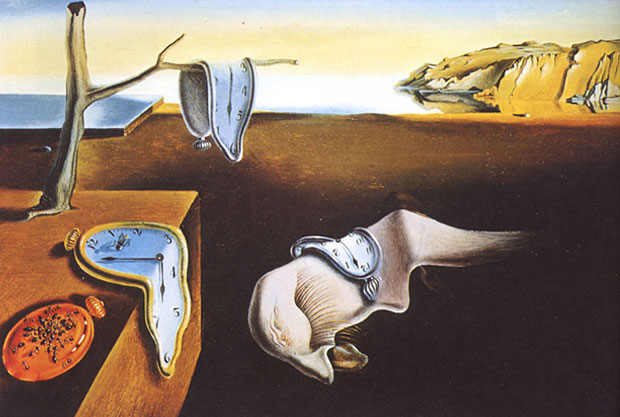
\includegraphics[width=1.3\textwidth]{Im/persistenceofmemory1931.jpg}
    \caption{\textit{La persistencia de la memoria}, de Salvador Dalí.}
    \label{fig:sen}
\end{marginfigure}

Apelando al Principio de Equivalencia, podemos decir que, si un sistema acelerado equivale a un espacio con una métrica particular que varía al hacer variar las coordenadas, entonces también \textbf{un campo gravitatorio es un cambio en la métrica del espacio-tiempo, determinado por las cantidades} $g_{\mu\nu}$. Ya estamos conectando la geometría del espacio-tiempo (su métrica) con fenómenos físicos (gravitación), independizándonos de las coordenadas (sistemas no-inerciales).

Aún nos falta definir un espacio-tiempo curvo, y para ello vamos a recordar la conclusión de la sección anterior: \textbf{un campo gravitatorio no puede eliminarse completamente tomando un sistema de referencia particular, sino que sólo podemos eliminarlo localmente}. Llevándolo al lenguaje del tensor métrico, \textbf{no existe transformación que lleve a $g_{\mu\nu}$ a una forma $\eta_{\mu\nu}$ (de Minkowski, o espacio-tiempo plano) para todo el espacio}. 
\begin{marginfigure}
\captionsetup{type=figure}
    \centering
    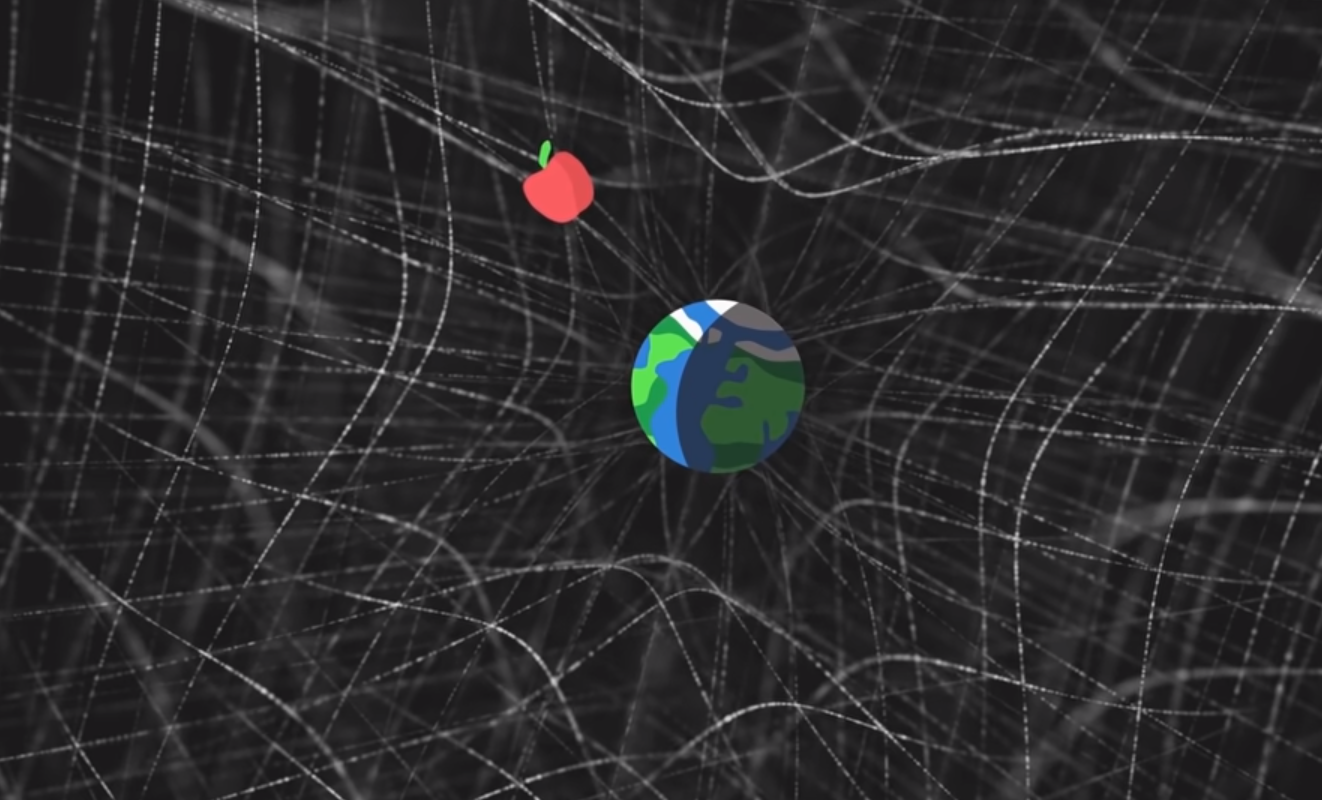
\includegraphics[width=1.3\textwidth]{Im/curve3d.png}
    \caption{Una manera de visualizar un espacio-tiempo curvo, que es conceptualmente más acertada, aunque no tan fácil de interpretar.}
    \label{fig:sen}
\end{marginfigure}

Y esta es justamente la definición de curvatura que vamos a utilizar\cite[][p.245]{landau2}:
\begin{remarkbox}{}
\textbf{Se dice que un espacio-tiempo está \textit{curvado} cuando su tensor métrico no puede reducirse al del espacio de Minkowski en todos lados}.
\end{remarkbox}
Como era de esperar, la curvatura es una \textbf{propiedad global} del espacio-tiempo, que puede aproximarse \textbf{localmente} por un espacio-tiempo plano (es decir, podemos eliminar la curvatura punto a punto), de la misma forma que la gravitación es una propiedad global del espacio-tiempo que puede eliminarse punto a punto eligiendo un sistema acelerado.

\subsection*{\textbf{Vectores Contravariantes y Covariantes}}

Ha llegado el momento de adentrarnos en el formalismo matemático propio de la Relatividad General. Como estamos interesadxs en cantidades que no dependan de los sistemas de coordenadas, vamos a definir muchos elementos \textit{según cómo transforman}. Si transformamos las coordenadas de las secciones anteriores, según la regla de la cadena se van a relacionar mediante:

\begin{equation}
    dx'^\mu=\frac{\partial x'^\mu}{\partial x^\nu}d x^\nu
\end{equation}

Si la base es una base curvilínea como las que vimos, las componentes $dx^\mu$ son en particular las componentes del desplazamiento $d\mathbf{s}$. Podemos entonces definir un \textbf{vector contravariante} $\mathbf{A}$, de modo tal que sus componentes se transformen como el desplazamiento $d\mathbf{S}$:

\begin{equation}
    A'^\mu=\frac{\partial x'^\mu}{\partial x^\nu}A^\nu
\end{equation}

Es posible ver que, si tomamos una función escalar de cuatro variables $\Phi$ y calculamos su gradiente $\partial_\mu \Phi$, este transformará de una forma distinta. En particular:

\begin{equation}
    \partial_\nu ' \Phi = \frac{\partial x^\mu}{\partial x'^\nu}\partial_{\nu}\Phi 
\end{equation}

Esto nos motiva a definir un \textbf{vector covariante}, cuyas componentes transforman como el gradiente $\partial_\mu \Phi$:

\begin{equation}
    B'_{\nu} = \frac{\partial x^\mu}{\partial x'^\nu}B_{\nu} 
\end{equation}

Combinando estos dos tipos de vectores, podemos construir tres tipos distintos de tensores:

\begin{remarkbox}{Tensores}
\begin{itemize}
    \item \textbf{Tensor contravariante} $A^{\mu\nu}$, cuyas componentes trasforman como los productos de las componentes de dos vectores contravariantes:
    
    $$A'^{\mu\nu}=\frac{\partial x'^\mu}{\partial x^\alpha}\frac{\partial x'^\nu}{\partial x^\beta}A^{\alpha \beta}$$
    
    \item \textbf{Tensor covariante} $A_{\mu\nu}$, cuyas componentes trasforman como los productos de las componentes de dos vectores covariantes:
    
    $$A'_{\mu\nu}=\frac{\partial x^\alpha}{\partial x'^\mu}\frac{\partial x^\beta}{\partial x'^\nu}A_{\alpha \beta}$$
    
    \item \textbf{Tensor mixto} $A^{\mu\nu}$, cuyas componentes trasforman como los productos de las componentes de dos un vector contravariante con uno covariante:
    
    $$A'^{\mu}_\nu=\frac{\partial x'^\mu}{\partial x^\alpha}\frac{\partial x^\beta}{\partial x'^\nu}A^{\alpha}_{\beta}$$
\end{itemize}
\end{remarkbox}

\newpage

\section{\huge{Cálculo de Curvatura}}
\textcolor{myred}{\hrule}

\newthought{Como introdujimos al hablar de curvatura}, un campo gravitatorio queda completamente descripto por la variación de un tensor métrico $g_{\mu\nu}$. Ahora bien, ¿cómo representamos dicha variación?. Un primer intento podría ser tomando el gradiente del tensor, de manera análoga a como tomamos el gradiente de un escalar para definir los covectores. Si tomamos un vector $A^\mu$ y calculamos su gradiente, conseguiremos una expresión de la forma $\partial_{\nu}A^{\mu}$. Si queremos transformarlo, tenemos que (utilizamos derivada del producto y definición de gradiente):

\begin{equation}
    \partial'_{\nu}A'^{\mu}=\frac{\partial x^{\beta}}{\partial x'^{\nu}}\frac{\partial^2 x'^\mu}{\partial x^\beta \partial x^\alpha}A^{\alpha}+\frac{\partial x^\beta}{\partial x'^\nu}\frac{\partial x'^{\mu}}{\partial x^{\alpha}}(\partial_\beta A^{\alpha})
\end{equation}

Si sólo tuviéramos el segundo término del lado derecho, entonces esta cantidad transformaría como un tensor, pero si los factores de transformación de coordenadas $\partial dx'^{\mu}/\partial d x^{\nu}$ no son constantes, entonces las derivadas segundas del primer término podrían no anularse. Esto quiere decir que las componentes del gradiente de un vector generalmente \textit{no} transforman como un tensor. Como hemos definido a los tensores según cómo transforman los vectores contravariantes y covariantes, lo mismo sucederá con el gradiente de un tensor, es decir que \textbf{el gradiente de un tensor no es un tensor}. Esto es un problema, ya que queremos construir una teoría con cantidades tensoriales, porque son independientes del sistema de referencia.

\subsection*{\textbf{Derivadas Primeras del Tensor Métrico}}

Para solucionar esto, pensemos en el caso más sencillo posible: un campo vectorial que es constante en todo el espacio. El gradiente 'verdadero' de este campo debería ser cero, y evidentemente en un sistema de coordenadas cartesiano, $\partial_{\mu}A^{\mu}=0$. Pero si tomamos un sistema de coordenadas curvilíneo, debemos tomar en cuenta las variaciones de los propios vectores de la base (los $\mathbf{e}_{\mu}$), que generalmente serán distintas de cero. 

\begin{marginfigure}
\captionsetup{type=figure}
    \centering
    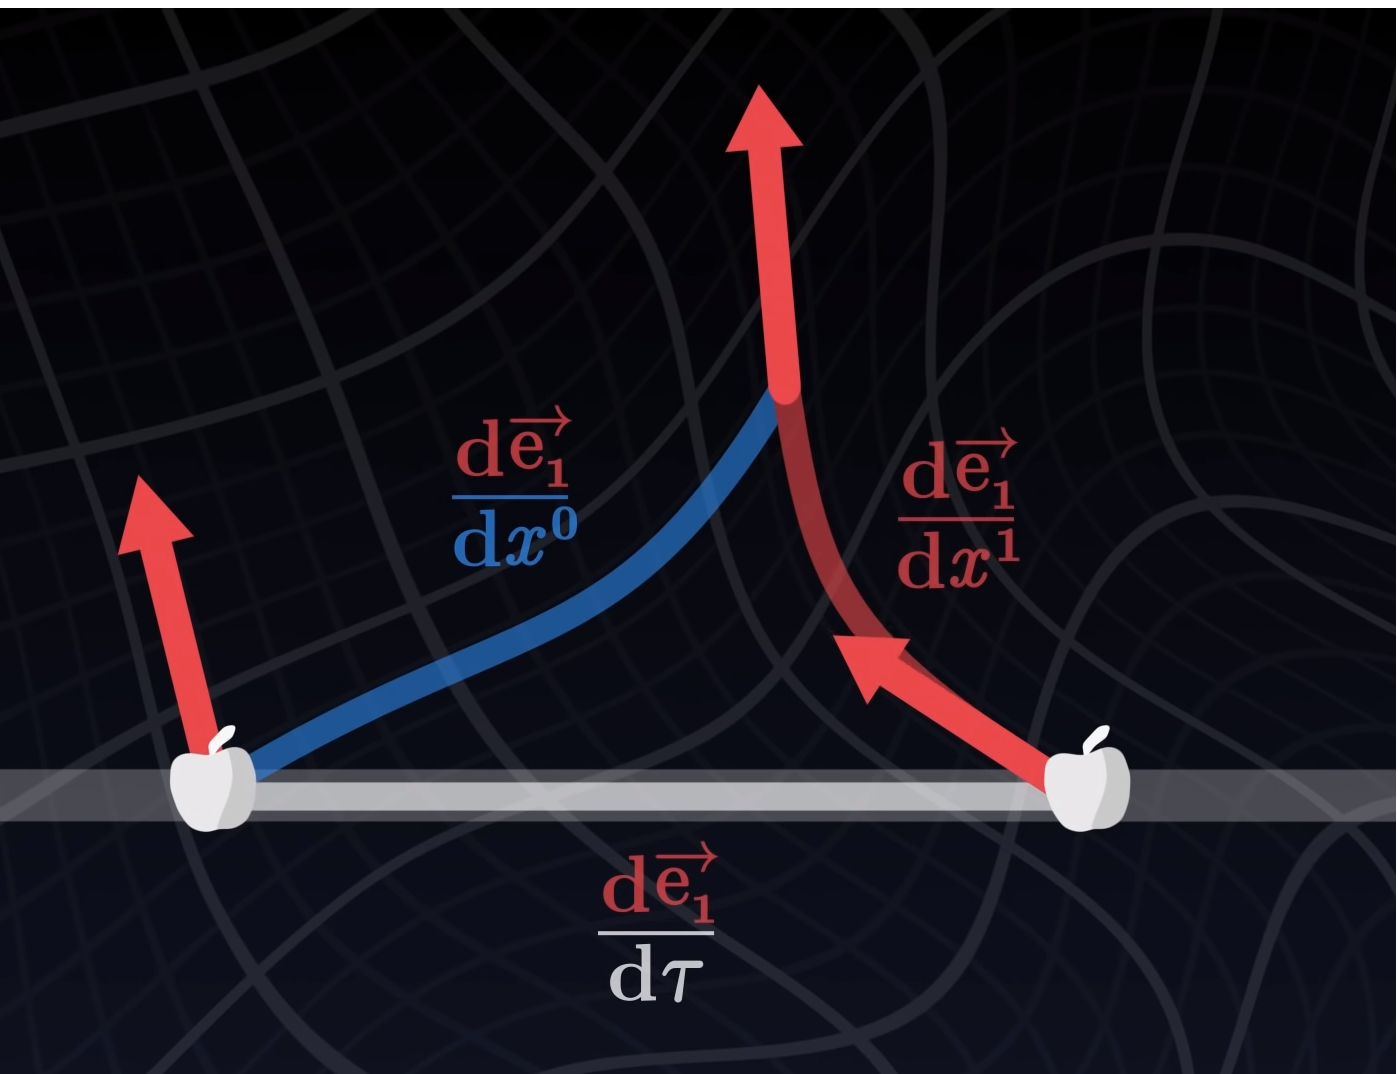
\includegraphics[width=1.3\textwidth]{Im/cambiocoord.png}
    \caption{Al estudiar la variación de un campo vectorial con coordenadas curvilíneas, debemos considerar el cambio del propio campo vectorial, y también el cambio de los vectores de la base.}
    \label{fig:sen}
\end{marginfigure}

Tomemos entonces un vector $\mathbf{A}(x^\mu)$, y veamos cómo varía al desplazarlo una cantidad infinitesimal $d\mathbf{s}$, de componentes $dx^\mu$:

\begin{equation}
d\mathbf{A}=d(A^\mu \mathbf{e}_{\mu})=\left(\frac{\partial A^{\mu}}{\partial x^{\sigma}}dx^\sigma \right)\mathbf{e}_{\mu}+A^\mu\frac{\partial \mathbf{e}_{\mu}}{\partial x^\alpha}dx^\alpha
\end{equation}

Vemos entonces que el primer término está relacionado a la variación del vector $\mathbf{A}$ al movernos en el espacio una cantidad $dx^{\mu}$, mientras que \textbf{el segundo término viene de la propia variación de los vectores de coordenadas curvilíneas}. Esto nos motiva a realizar dos definiciones nuevas:

\begin{remarkbox}{Símbolos de Christoffel}
Para un dado punto $\mathcal{P}$ en un espacio-tiempo con vectores de base $\mathbf{e}_{\mu}$, definimos los símbolos de Christoffel como los coeficientes $\Gamma^\nu_{\mu\alpha}$ que satisfacen:

\begin{equation}
    \frac{\partial \mathbf{e}_{\alpha}}{\partial x^{\mu}}\equiv \Gamma^\nu_{\mu\alpha} \mathbf{e}_{\nu}
\end{equation}

\end{remarkbox}

\begin{marginfigure}
\captionsetup{type=figure}
    \centering
    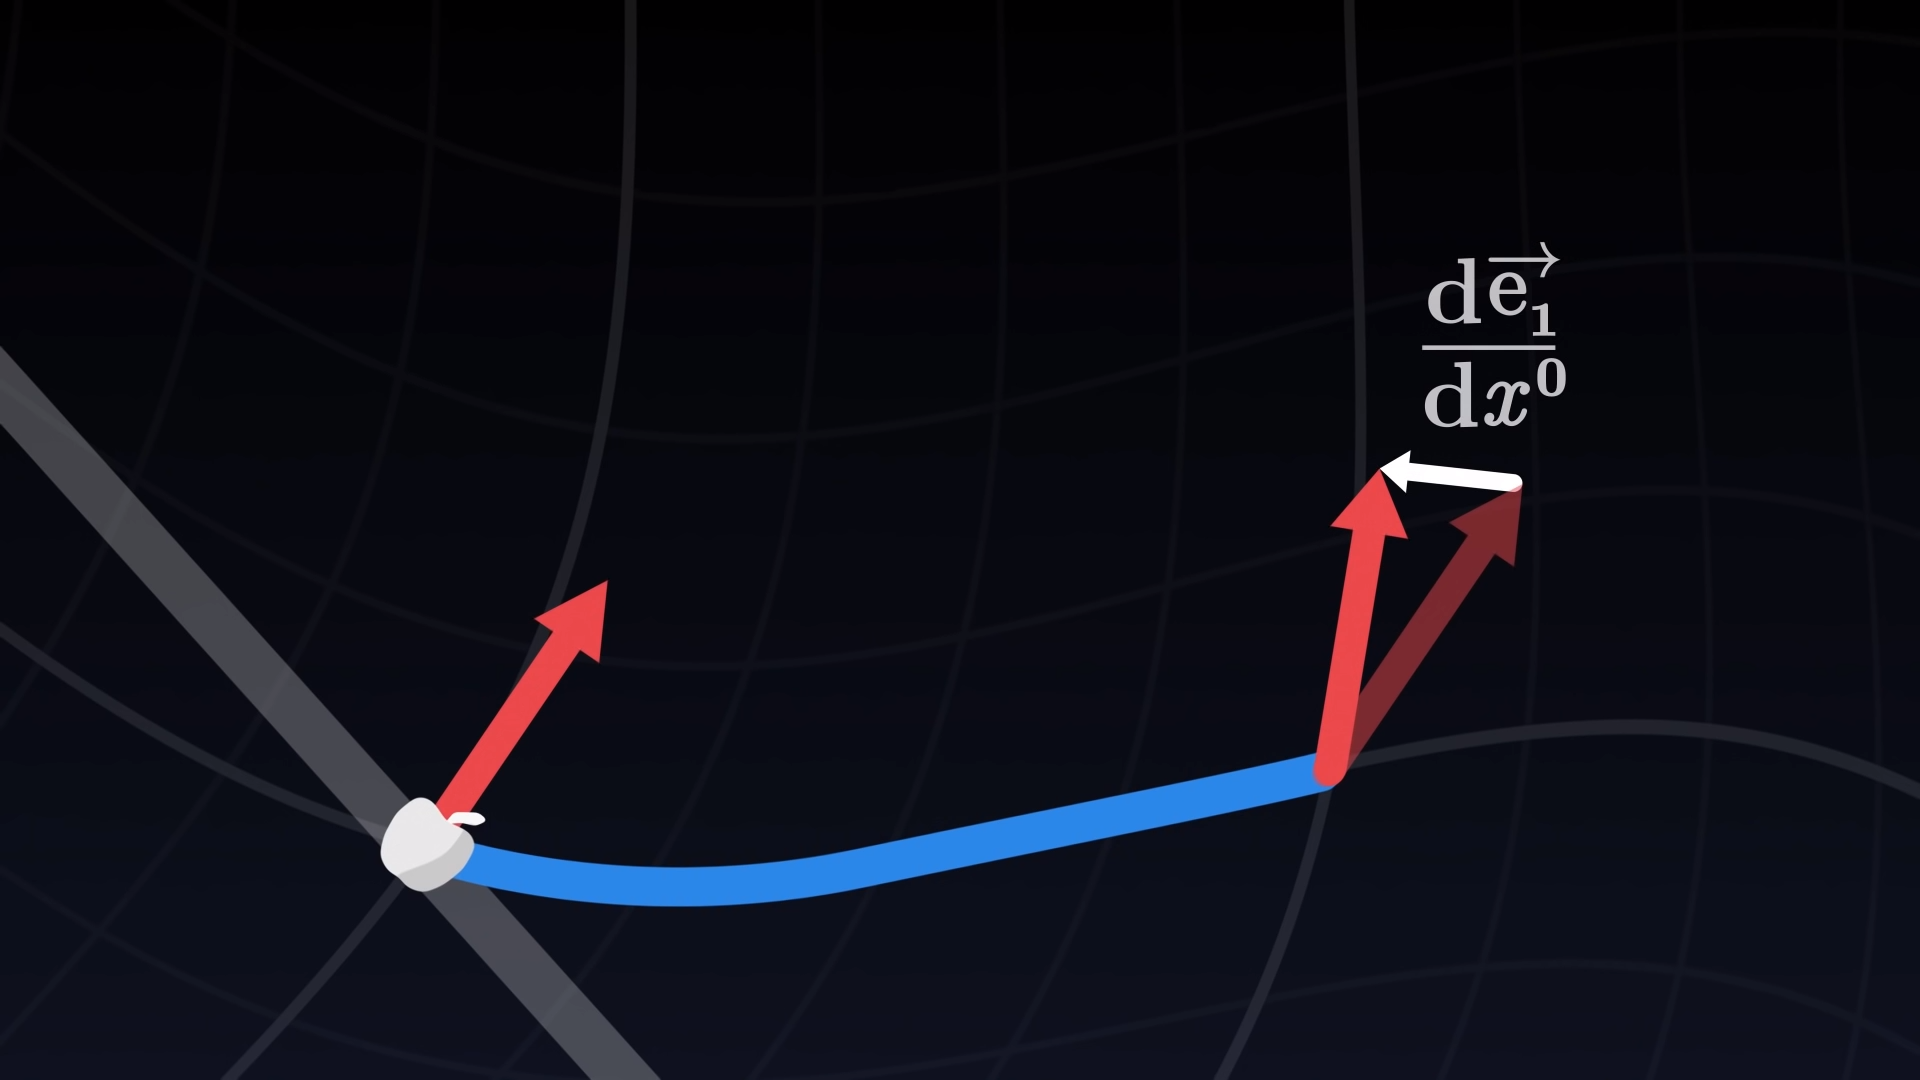
\includegraphics[width=1.3\textwidth]{Im/parallel.png}
    \caption{Transporte paralelo de un vector. Restando los vectores de cada punta obtenemos cómo cambia uno de los vectores de la base al variar la otra coordenada.}
    \label{fig:sen}
\end{marginfigure}

\begin{marginfigure}
\captionsetup{type=figure}
    \centering
    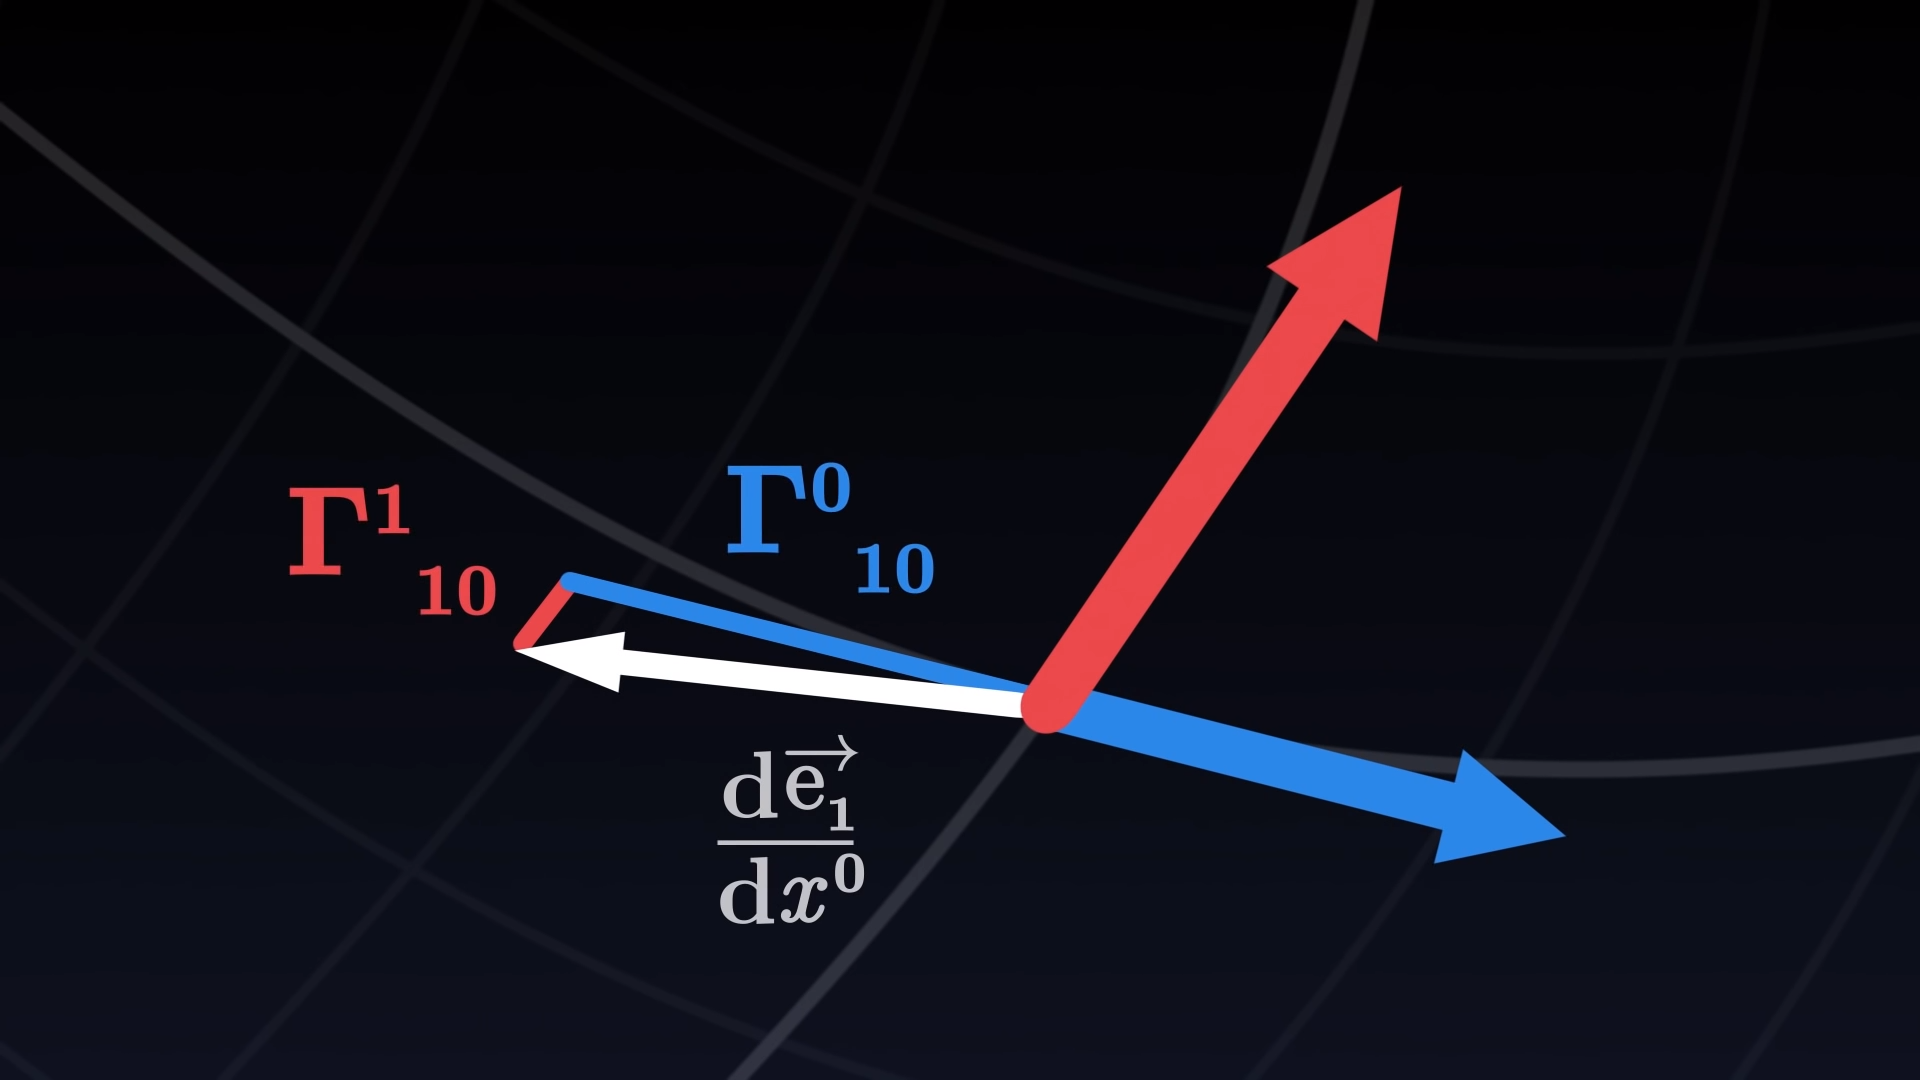
\includegraphics[width=1.3\textwidth]{Im/christoffel.png}
    \caption{Los símbolos de Christoffel representan cómo cambian los vectores de la base al desplazarnos en el mismo espacio, en las mismas coordenadas que estamos utilizando. Necesitamos tres índices, porque uno representa cuál es el vector $\mathbf{e}_{\mu}$ que estamos estudiando, otro indica cuál es la coordenada $x^{\nu}$ que hicimos variar, y el último cuál es la componente de la propia variación.}
    \label{fig:sen}
\end{marginfigure}

\begin{marginfigure}
\captionsetup{type=figure}
    \centering
    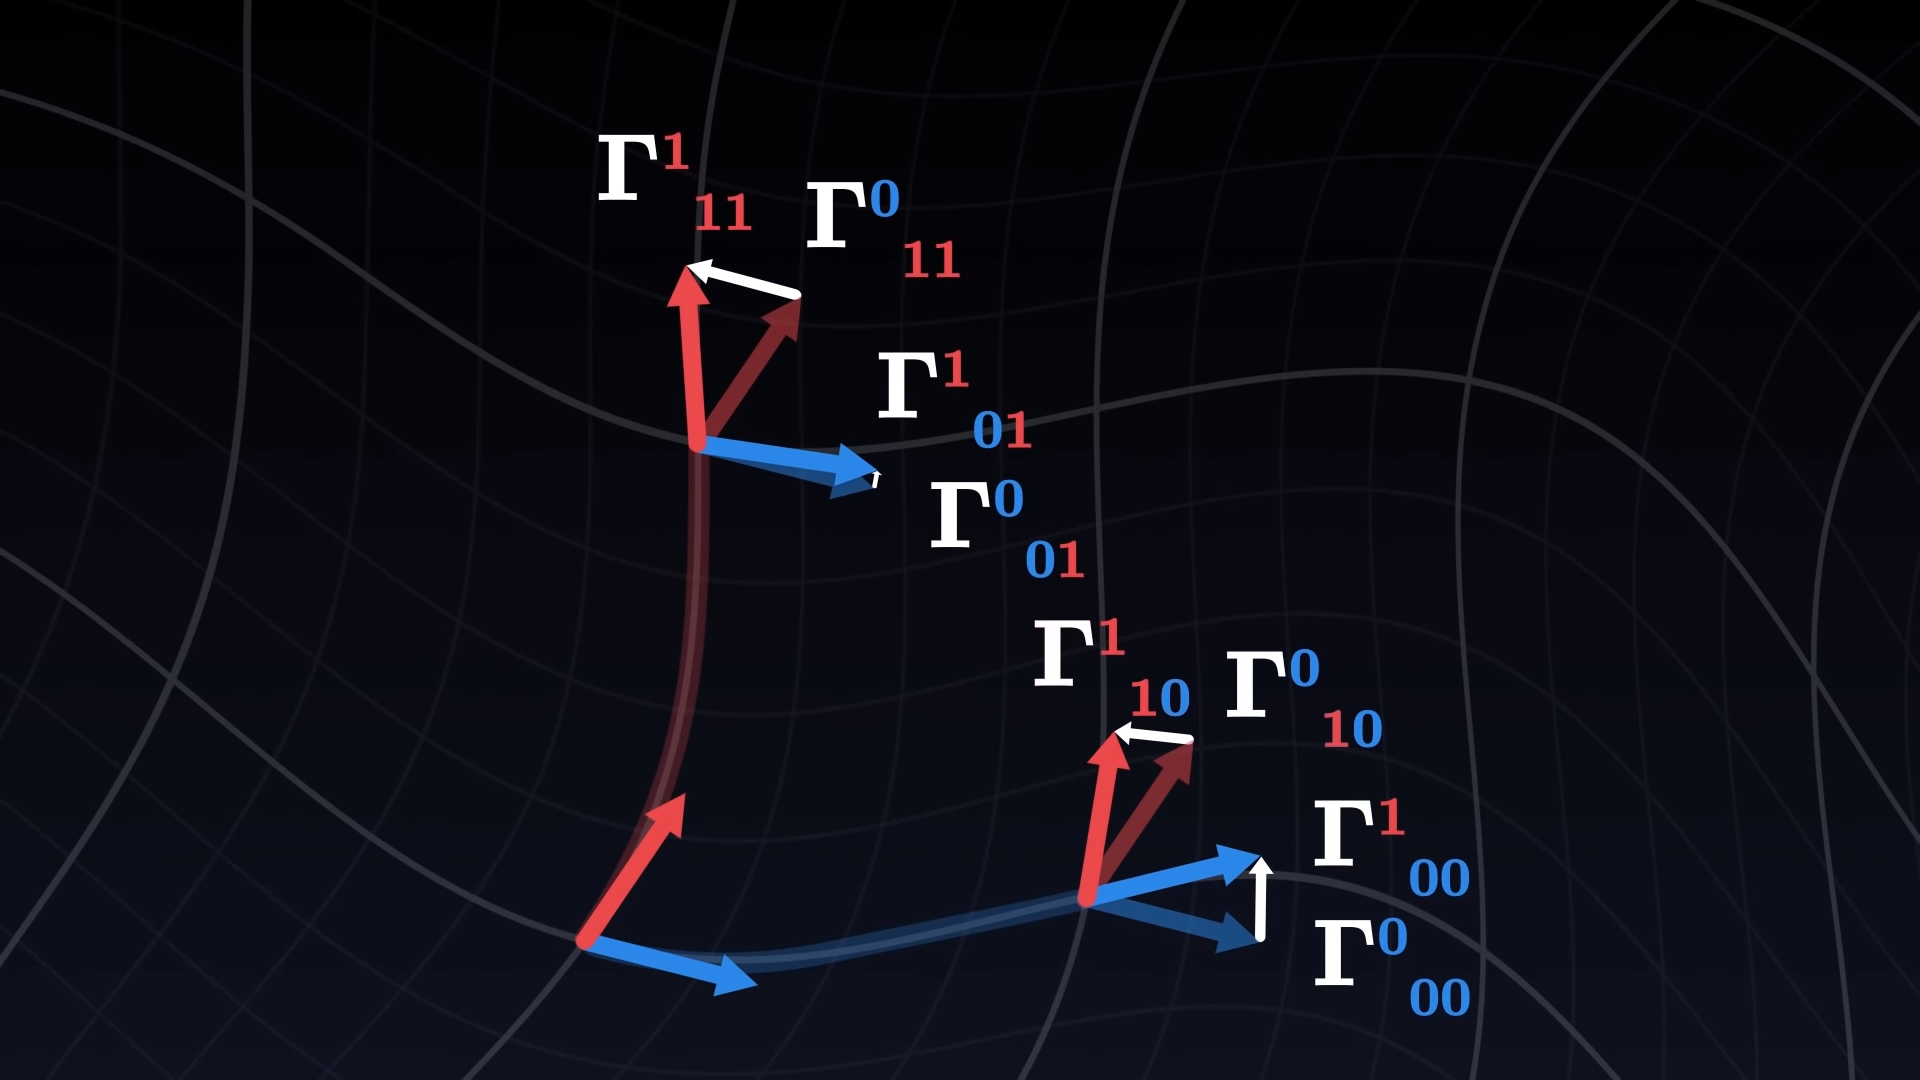
\includegraphics[width=1.3\textwidth]{Im/muchoscristoffel.png}
    \caption{En dos dimensiones, hay 8 símbolos de Christoffel para cada punto del espacio, de los cuales 6 son independientes.}
    \label{fig:sen}
\end{marginfigure}

Utilizando estos símbolos, podemos escribir a la ecuación para $d\mathbf{A}$ como:

\begin{equation}
    d\mathbf{A}= \left[\frac{\partial A^{\mu}}{\partial x^\alpha}+\Gamma^\mu_{\alpha \nu}A^{\nu}\right]\mathbf{e}_{\mu}dx^{\alpha}
\end{equation}

\begin{remarkbox}{Gradiente Absoluto (para un vector)}
        Definimos ahora el gradiente absoluto o derivada covariante de un campo vectorial $\mathbf{A}(x^{\alpha})$ según:
        
        \begin{equation}
            \nabla_\alpha A^{\mu}\equiv\frac{\partial A^{\mu}}{\partial x^\alpha}+\Gamma^\mu_{\alpha \nu}A^{\nu}
        \end{equation}
\end{remarkbox}


El gradiente absoluto es justamente la cantidad que estábamos buscando: un tensor que representa cómo varían los vectores al movernos en un espacio-tiempo curvo.

También podemos escribir, de manera análoga, el gradiente absoluto de un tensor:

\begin{remarkbox}{Gradiente Absoluto (para un tensor)}
\begin{equation}
\nabla_\gamma T^{\alpha\beta} = \partial_\gamma T^{\alpha\beta} + \Gamma^\alpha_{\mu\gamma}T^{\mu\beta} + \Gamma^\beta_{\mu\gamma}T^{\alpha\mu}
\end{equation}
\end{remarkbox}

Por otro lado, podemos interpretar los símbolos de Christoffel como sigue: realizamos el \textbf{transporte paralelo} de un vector, que significa desplazar un vector de forma paralela a sí misma, de modo tal que en coordenadas cartesianas conseguiríamos el mismo vector. Como estamos en coordenadas curvilíneas, los vectores aquí sí varían.


Ahora tomamos la variación del vector al realizar el transporte paralelo, y lo descomponemos en las componentes según los vectores de la base en ese mismo punto. Estas componentes son los símbolos de Christoffel.

Los símbolos de Christoffel son \textbf{simétricos} en sus dos índices inferiores, lo cual reduce la cantidad de símbolos independientes de 64 a 40. 

Además, si tomamos la definición de los símbolos de Christoffel y hacemos el producto escalar con algún otro vector de la base, podemos establecer una relación entre los $\Gamma^{\alpha}_{\mu \nu}$ y el tensor métrico. Esta es:

\begin{remarkbox}{}
\begin{equation}
    \Gamma^{\alpha}_{\mu \nu}=\frac{1}{2}g^{\alpha\sigma}\left[\partial_{\mu}g_{\nu\sigma}+\partial_{\nu}g_{\sigma \mu}-\partial_{\sigma}g_{\mu\nu}\right]
    \label{simboloChristoffel}
\end{equation}
\end{remarkbox}

Donde $g^{\alpha\sigma}$ es la \textbf{inversa} del tensor métrico (en el sentido matricial de inversa), es decir que $g^{\alpha\sigma}g_{\sigma\beta}=\delta^{\alpha}_\beta$.

\vspace{0.5cm}

Perfecto, ya tenemos una cantidad asociada a la variación del tensor métrico, ¿estamos en condiciones de expresar la curvatura del espacio-tiempo matemáticamente? \textbf{No}. Si hacemos memoria, localmente podemos aproximarnos a todo punto mediante un sistema cartesiano, cuya métrica es $\eta_{\mu\nu}$. Es decir que, además de reducir la métrica a la del espacio plano, también tenemos que, en ese punto, $\partial_\alpha g_{\mu\nu}=0$. No sólo eso, sino que además, en estos sistemas (llamados \textbf{localmente inerciales}), el gradiente absoluto se reduce al gradiente ordinario (por ser sistemas cartesianos), y entonces:

\begin{equation}
    \nabla_{\alpha}g_{\mu\nu}=\partial_\alpha g_{\mu\nu}=0
\end{equation}

Notemos que esta última es una ecuación tensorial, es decir que es independiente del sistema de coordenadas, de donde concluimos que \textbf{el gradiente absoluto del tensor métrico es nulo en todo sistema de referencia}.

\subsection*{\textbf{Derivadas Segundas del Tensor Métrico}}

Resulta que la verdadera información sobre la curvatura de un espacio-tiempo yace en las derivadas de segundo orden. Mediante un análisis de \textbf{desviaciones geodésicas}\cite[][p.211]{moore} (que aquí se ha omitido), podemos construir el llamado \textbf{Tensor de Riemann}, del cual daremos la definición y sus características fundamentales.

\begin{remarkbox}{Tensor de Riemann}
        Definimos al tensor de Riemann $R^\alpha_{\mu \nu \sigma}$ según:
        \begin{equation}
            R^\alpha_{\mu \nu \sigma}\equiv\partial_{\nu}\Gamma^{\alpha}_{\mu \nu}-\partial_{\sigma}\Gamma^{\alpha}_{\mu\sigma}+\Gamma^{\alpha}_{\mu\gamma}\Gamma^{\gamma}_{\mu\sigma}-\Gamma^{\alpha}_{\sigma\gamma}\Gamma^{\gamma}_{\mu\nu}
            \label{riemann}
        \end{equation}
        
        Sobre él podemos decir:
        \begin{itemize}
            \item Tiene 256 entradas, pero debido a las muchas simetrías del mismo, sólo 20 son independientes.
            \item Es \textbf{nulo para espacios planos}, y \textbf{no nulo para espacios curvados}, lo que lo hace la herramienta ideal para analizar la curvatura del espacio estudiado.
        \end{itemize}
\end{remarkbox}

Vamos a definir también otras cantidades que nos resultarán útiles a la hora de armar las Ecuaciones de Campo de Einstein.

\begin{remarkbox}{Tensor de Ricci}
        Definimos al tensor de Ricci $R_{\beta\nu}$ como la \textbf{contracción} del tensor de Riemann sobre su primera y tercera componente:
        \begin{equation}
            R_{\beta\nu} \equiv R^\alpha_{\beta \alpha \nu} \equiv g^{\alpha \mu} R_{\alpha\beta\mu\nu}
            \label{ricci}
        \end{equation}
        
        Este tensor es simétrico, y tiene 10 entradas independientes.
\end{remarkbox}

\begin{remarkbox}{Escalar de Curvatura}
        A su vez, definimos el escalar de Ricci o escalar de curvatura $R$ como la contracción del tensor de Ricci:
        \begin{equation}
            R \equiv g^{\beta\mu}R_{\beta\mu}\equiv g^{\beta\mu}g^{\alpha \mu} R_{\alpha\beta\mu\nu}
        \end{equation}
        
        Es interesante porque esta cantidad es un \textbf{escalar relativista}, es decir su valor no depende de la elección de coordenadas.
        
        Si $R_{\beta\nu} \neq 0$ o $R\neq 0$, ya podemos asegurar que el espacio está curvado, mientras que el recíproco no siempre es válido.
\end{remarkbox}


